%%%%%%%%%%%%%%%%%%%%%%%%%%
%% Template file for an IEE conference article
%% Trim Size: A4 Paper
%% iiai-conference.tex   :   29-2-08
%% Tex file to use with iiai-c.sty written in Latex2E.
%% The content, structure, format and layout of this style file is the
%% property of International Institute of Applied Informatics
%% Copyright 2013 by International Institute of Applied Informatics
%% All rights are reserved.
%% Created by Satoshi Takahashi, UEC, Japan, Antoine Bossard, AIIT, Japan, Wen Gu, JAIST, Japan and Shun Okuhara, Mie University, Japan
%%%%%%%%%%%%%%%%%%%%%%%%%%
\documentclass[11pt, onecolumn, twoside, a4paper]{article}
\usepackage{iiai-c}
%\usepackage{} % for times new roman; Antoine will send email
\usepackage{graphicx}
\usepackage{amsmath}
\usepackage{amssymb}
\usepackage{amsthm}
\usepackage{lipsum}
\usepackage{mathptmx}
\usepackage{comment}
\usepackage[rm,up,sc,topmarks,calcwidth,pagestyles]{titlesec}
\titleformat{\section}{\Large\bfseries\rmfamily}{\thesection}{1em}{}
\titleformat{\subsection}{\large\bfseries\rmfamily}{\thesubsection}{1em}{}
\titleformat{\subsubsection}{\large\it\rmfamily}{\thesubsubsection}{1em}{}

\newtheorem{theorem}{Theorem}
\newtheorem{lemma}[theorem]{Lemma}
\newtheorem{corollary}[theorem]{Corollary}
\newtheorem{property}[theorem]{Property}
\newtheorem{define}[theorem]{Definition}
\newtheorem{assume}[theorem]{Assumption}
\def \Re {\mathbb{R}}


% Edit by IEE editor
\authorshead{S.~Takahashi, A.~Bossard, T.~Matsuo, T.~Fukushima}
\titlehead{IIAI Open Conference Publication Series {\LaTeX} Template}
\vol{1}
\no{1}
\year{2015}
\setcounter{page}{48} % edit
\page{48}
\lastpage{62} % edit


\title{A Platform for Searching Texts for Desired Expressions in a User-editable Pattern Matching Environment for Language Learning}
\author{Tatsuya Katsura \thanks{Graduate School of Environmental, Life, Natural Schience and Technology, Okayama University, Okayama, Japan}, Koichi Takeuchi \thanks{Faculty of Environmental, Life, Natural Science and Technology, Okayama University, Okayama, Japan} }
\date{}  
\begin{document}
\maketitle
\thispagestyle{empty}

\section*{Abstract}
In this paper we propose a platform of pattern matching system that can extract required phrases or sentences in texts.
Finding certain expressions in texts are often needed in language learning, e.g, examples of case markers
between a predicate and an argument, or possible nouns in subject of a verb in a certain meaning. In previous studies,
several types of systems, containing concordancers, are proposed; however, language learner

The concordancer used by language learners has fixed templeates of search patterns and user use it on them
less flexibility. 
the user want to apply othe type of pattern matching, they are reruied to build new program, but this is too cost.
Thus, we propose a platform of text searching system in which users can edit their search patterns
with complext  by combining blocks of basic search patterns. As a characteristics advantage of the proposed
system is user can also designate the highligting part in texts, e.g, phrase or words,
with the combination block pattern. To realize the pattern matching of predicate-argument structure,
the system emplopys several NLP tools. In performance test, experimental results show architecture of system 
thanks to the architecture, our system deal with large sclale texts (10,000 texts) because of database system. 


by devising architecture 
In this paper we discuss the 

and display parts, and the degree of freedom is limited. In order to create more free patterns, it is necessary to create them by program, but it is not easy because it requires skills different from language learning. Therefore, in this study

it is 
a
is used and developed
containing concordancer as a tool
requested
very flexible is 

however, 

to find some expressions in texts.
necessary to find the required expressions in the text.

thus in this paper we propose flexible sytem of
with pattern matching system of 

These instructions give you guidelines for preparing papers for IIAI Open Conference Publication Series. Use this document as a template if you are using {\LaTeX}. Otherwise, use this document as an instruction set. The electronic file of your paper will be edited further at IIAI. Define all symbols used in the abstract. Do not cite references in the abstract. Do not delete the blank line immediately above the abstract. Use only English to write a paper.  
%
%\section*{Keywords}
%About four key words or phrases in alphabetical order, separated by commas.
%
%\noindent
\\[2mm]
{\it Keywords: }About four key words or phrases in alphabetical order, separated by commas.


\section{Introduction}

This document is a {\LaTeX} template for IIAI Open Conference Publication Series. 
If you prefer to use Microsoft Word, please download the file from the conference webpage.
{\bf Do not change the font sizes or line spacing to squeeze more text into a limited number of pages. }
Use italics for emphasis; do not underline.  
The page limit is defined separately for each volume. Please do not exceed the page limit. 

\section{Copyright}
An IIAI electronic copyright form should accompany your final submission or registration of the conference. The instruction of copyright transfer is announced at the conference webpage. Authors are responsible for obtaining any security clearances for the copyright form submission.


\section{Figures and Tables}
To insert images in the paper, use outlined .eps/.pdf file of high resolution.  
Each figure should have a caption giving a brief explanation of the figure. 
If the figure includes copyrighted images, the author needs to get permission from copyright holders. 
Figure axis labels are often a source of confusion. Use words rather than symbols. 
If the image includes non-English word or symbols, explain their meanings. 
Each table should also have a caption. 

\begin{comment}
\begin{figure}[htbp]
  \begin{center}
    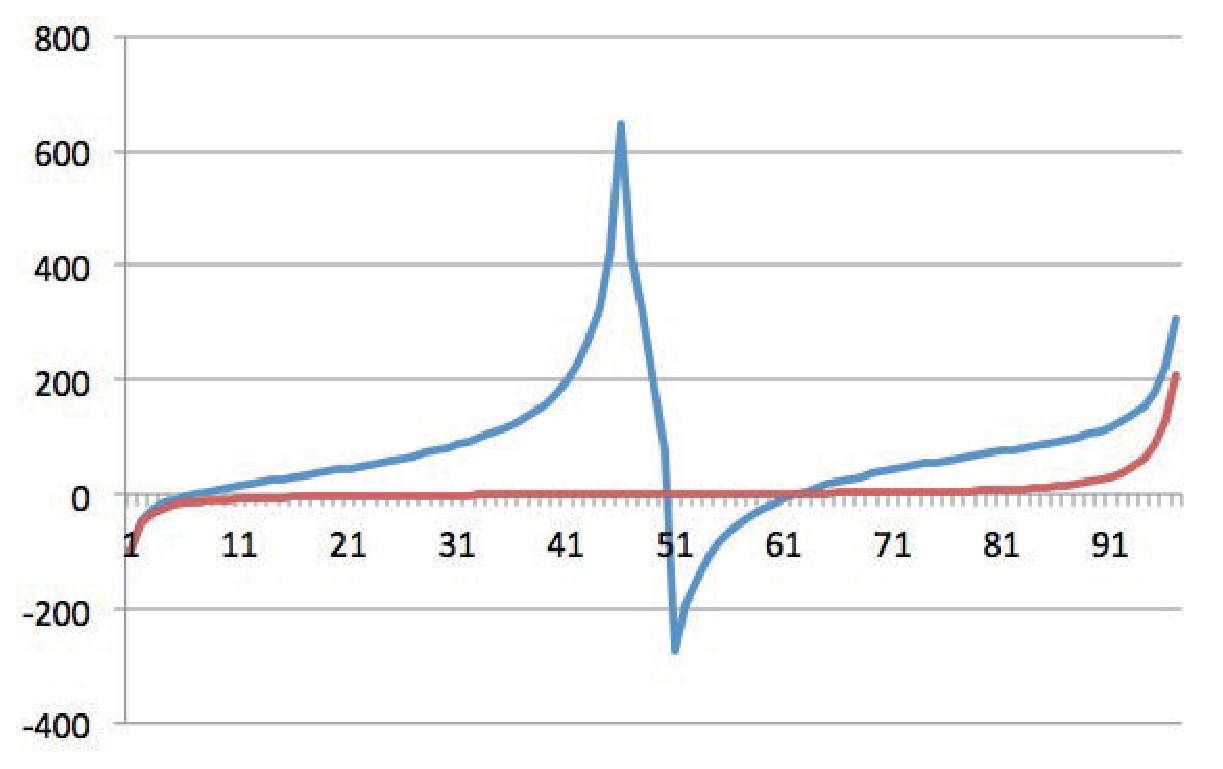
\includegraphics[clip,width=10.0cm]{./fig1.eps}
    \caption{Example}
    \label{fig:example}
  \end{center}
\end{figure}
\end{comment}
Because IIAI will do the final editing formatting of your paper, 
you do not need to pay much attention to figures and tables position. 
Large figures and tables may be divided into multiple figures. 
Place figure captions below the figures; place table titles above the tables. 
If your figure has two parts, include the labels ``(a)'' and ``(b)'' as part of the artwork. 
Please verify that the figures and tables you mention in the text actually exist. 
Please do not include captions as part of the figures. 
Do not put captions in ``text boxes'' linked to the figures. 
Do not put borders around your figures. 
Please do not abbreviate ``Figure'' and ``Table'' like ``Fig'' and ``Tbl'' in the text. 

Figures in print will appear in grayscale (black and white), though the full color version will appear in the electronic version of your published manuscript. Any copyrighted image must include indication in the caption of the original source of the image and that it is being used with permission of the copyright holder. Authors may have to pay the permission fee when the copyright holder of the image requires it.




\section{References}

Number citations consecutively in square brackets \cite{1}. 
The sentence punctuation follows the brackets \cite{2}. 
Multiple references are each numbered with separate brackets \cite{1}\cite{2}\cite{3}. 
When citing a section in a book, please give the relevant page numbers. 
In sentences, refer simply to the reference number, as in \cite{3}. 
Do not use ``Ref. \cite{3}'' or ``reference \cite{3}'' except at the beginning of a sentence: ``Reference \cite{3} shows ... .'' 
Do not put citations and references in footnotes. 
References in the references list should appear in the order of appearance in the paper. 
Give all authors’ names; do not use ``et al.'' unless there are six authors or more. 
Use a space after authors' initials. 
Papers that have not been published should be cited as ``unpublished'' [4]. 
Papers that have been submitted for publication should be cited as ``submitted for publication'' [5]. 
Papers that have been accepted for publication, but not yet specified for an issue should be cited as ``to be published'' [6]. 
Please give the URL and the date of access for webpage citation [7].
Capitalize only the first word in a paper title, except for proper nouns and element symbols. 
For papers published in translated journals, please give the English citation first, followed by the original foreign-language citation [8]. If the papers are 
published in non-English languages, translate the paper title and journal name. IIAI does not recommend to refer non-English language publications. 
IIAI journals employ IEEE transaction reference style. 


\subsection{Example}
\subsubsection{Article in a collection}
[1] A.J. Albrecht, ``Measuring Application-Development Productivity,'' Programmer Productivity Issues for the Eighties, 2nd ed., C. Jones, ed., IEEE CS, 1981, pp. 34–43.
\subsubsection{Article in a conference proceedings}
[2] H. Yuan et al., ``Sparse Representation Using Contextual Information for Hyperspectral Image Classification,'' Proc. 2013 IEEE Conf. Cybernetics (CYBCONF 13), 2013, pp. 138–143.
\\[1mm]
[3] N. Zhong, ``Toward Web Intelligence,'' Advances in Web Intelligence: 1st Int'l Atlantic Web Intelligence Conf. (AWIC 03), LNCS 2663, 2003, pp. 1–14.
\subsubsection{Article in a journal or magazine}
[4] I.E. Sutherland, R.F. Sproull, and R.A. Schumaker, ``A Characterization of Ten Hidden-Surface Algorithms,'' ACM Computing Surveys, vol. 6, no. 1, 1974, pp. 1–55.
\subsubsection{Blog}
[5] M. Watson, Artificial Intelligence Blog; http://markwatson.com/aiblog.
\subsubsection{Book}
[6] W.M. Newman and R.F. Sproull, Principles of Interactive Computer Graphics, McGraw-Hill, 1979, p. 402.
\\[1mm]
[7] M.A. Arbib, ed., The Handbook of Brain Theory and Neural Networks, MIT Press, 1998.
\subsubsection{Book series}
[8] Y. Yao et al., ``Web Intelligence (WI): Research Challenges and Trends in the New Information Age,'' Web Intelligence: Research and Development, LNAI 2198, N. Zhong et al., eds., Springer, 2001, pp. 1-17. 
\\[1mm]
[9] R. Focardi and R. Gorrieri, eds., Foundations of Security Analysis and Design, LNCS 2171, Springer, 2001.
\subsubsection{CD}
[10] W.M. Newman and R.F. Sproull, Principles of Interactive Computer Graphics, CD-ROM, McGraw-Hill, 1979.
\\[1mm]
[11] William Song, ``A Semantic Approach to Internal Structure Formation in the Semantic Grid,'' Proc. Third Int'l Conf. Semantics, Knowledge, and Grid (SKG 2007), CD-ROM, IEEE CS, 2007, pp. 248-253.
\subsubsection{Dissertation or thesis}
[12] B. Fagin, ``A Parallel Execution Model for Prolog,'' PhD dissertation, Dept. Computer Sciences, Univ. of California, Berkeley, 1987.
\\[1mm]
[13] M. Nichols, ``The Graphical Kernel System in Prolog,'' master's thesis, Dept. Computer Science and Eng., Rensselaer Polytechnic Inst., 1985.
\subsubsection{Electronic publication(Article in a journal)}
[14] D. Kornack and P. Rakic, ``Cell Proliferation without Neurogenesis in Adult Primate Neocortex,'' Science; doi:10.1126/science.1065467.
\subsubsection{Electronic publication(Article in a conference proceedings)}
[15] H. Goto, Y. Hasegawa, and M. Tanaka, ``Efficient Scheduling Focusing on the Duality of MPL Representation,'' Proc. IEEE Symp. Computational Intelligence in Scheduling (SCIS 07), IEEE, 2007; doi:10.1109/SCIS.2007.367670.
\subsubsection{Electronic publication(Online-only publication)}
[16] F. Kaplan, ``From Baghdad to Manila: Another Lousy Analogy for the Occupation of Iraq,'' Slate, 21 Oct. 2003; http://slate.msn.com/id/2090114.
\subsubsection{Electronic publication(Website)}
[17] R. Bartle, ``Early MUD History,'' Nov. 1990; www.ludd.luth.se/aber/mud-history.html.
\subsubsection{Patents}
[18] M. Hoff, S. Mazor, and F. Faggin, Memory System for Multi-Chip Digital Computer, US patent 3,821,715, to Intel Corp., Patent and Trademark Office, 1974.
\subsubsection{Pending publication(Article)}
[19] R. Lee, ``New-Media Processing,'' to be published in IEEE Micro, Nov./Dec. 2012.
\subsubsection{Pending publication(Book)}
[20] R. Lee, Writing New Programs, McMillan, to be published in 2012.
\subsubsection{Preprint}
[21] J.M.P. Martinez et al., ``Integrating Data Warehouses with Web Data: A Survey,'' IEEE Trans. Knowledge and Data Eng., preprint, 21 Dec. 2007, doi:10.1109/TKDE.2007.190746.
\subsubsection{White paper}
[22] Consolidating the IT Infrastructure, white paper, Oracle Corp., Dec. 2003.



\subsection{Abbreviations in References}

If you prefer, you may use the following abbreviations in the titles of periodicals and when naming publishing institutions:

\begin{table}[hbtp]
 \caption{Abbreviations}
 \label{table:data_type}
 \begin{center}
  \begin{tabular}{ll}
   \hline
   Abbreviations & Word  \\
   \hline \hline
Conf. & Conference (on)\\
Dept.  & Department (of) \\
ed. & edition, editor\\
Inst. & Institute\\
Int'l & International\\
Nat'l & National\\
No. & Number\\
Org. & Organization\\
Proc. & Proceedings (of)\\
Symp. & Symposium (of or on)\\
Univ. & University\\
Vol. & Volume\\
   \hline
  \end{tabular}
 \end{center}
\end{table}




\section{Some Common Mistakes}

Do not use the word which has plural meaning. 
Use the word ``micrometer'' instead of ``micron.'' 
A graph within a graph is an ``inset,'' not an ``insert.'' 
The word ``alternatively'' is preferred to the word ``alternately'' (unless you really mean something that alternates). 
Use the word ``whereas'' instead of ``while'' (unless you are referring to simultaneous events). 
Do not use the word ``essentially'' to mean ``approximately'' or ``effectively.'' 
Do not use the word `issue'' as a euphemism for ``problem.'' 
Be aware of the different meanings of the homophones `affect'' (usually a verb) and ``effect'' (usually a noun), ``complement'' and ``compliment,'' ``discreet'' and ``discrete,'' ``principal'' (e.g., ``principal investigator'') and ``principle'' (e.g., ``principle of measurement''). Do not confuse ``imply'' and ``infer.'' 
Prefixes such as `non,'' ``sub,'' ``micro,'' ``multi,'' and ``ultra'' are not independent words; they should be joined to the words they modify, usually without a hyphen. 
There is no period after the ``et'' in the Latin abbreviation ``et al.'' (it is also italicized). 
The abbreviation ``i.e.,'' means ``that is,'' and the abbreviation ``e.g.,'' means ``for example'' (these abbreviations are not italicized). 



\section{Editorial Policies for General Issues}

\subsection{General Issues/Special Issues (Non Conference Related Papers)}

Submission of a manuscript is not required for presentation/participation in a conference. 
Do not submit a reworked version of a paper you have submitted or published elsewhere. 
The submitting author is responsible for obtaining the agreement of all coauthors and any consent required from sponsors before submitting a paper. IIAI Journals strongly discourage courtesy authorship. 
It is the obligation of the authors to cite relevant prior work. 
At least three to four reviewers are required for every paper submitted. 
Undecipherable English is a valid reason for rejection. 


\subsection{Special Issues (Conference Related Papers)}

For conference-related papers, the decision to accept or reject a paper is made by the guest editors of the special issues. Guest editors may be appointed by conference organizing committees. 
Do not submit a reworked version of a paper you have submitted or published elsewhere. 
Conference paper should be extended/improved from the original version. 
The extended/improved version should include at least 10 references. 
Undecipherable English is a valid reason for rejection. 
Authors of rejected papers may revise and resubmit them to an IIAI journal as regular papers, whereupon they will be reviewed by three to four new referees. 



\section{Publication Principle}

This publication principle is created based on IEEE transaction publication policies. 
Authors should consider the following points. 
Except for the papers which were already reviewed by technical committees, each submitted paper will be reviewed rigorously.

\subsection{Technical Papers}

\noindent
{\bf (1)  Novelty and relevancy:} Technical papers submitted for publication must advance the state of knowledge and must cite relevant prior work. 

\noindent
{\bf (2)  Page length and contents:} The length of a submitted paper should be commensurate with the importance, or appropriate to the complexity, of the work. For example, an obvious extension of previously published work might not be appropriate for publication or might be adequately treated in just a few pages.

\noindent
{\bf (3)  Significance of the work:} Authors must convince both peer reviewers and the editors of the scientific and technical merit of a paper; the standards of proof are higher when extraordinary or unexpected results are reported. 

\noindent
{\bf (4)  Information disclosure:} Because replication is required for scientific progress, papers submitted for publication must provide sufficient information to allow readers to perform similar experiments or calculations and use the reported results. Although not everything needs to be disclosed, a paper must contain new, useable, and fully described information. Authors should expect to be challenged by reviewers if the results are not supported by adequate data and critical details.

\noindent
{\bf (5)  Incomplete work:} Papers that describe ongoing work or announce the latest technical achievements, which are suitable for presentation at a professional conference, may not be appropriate for publication in a volume.





\section*{Acknowledgments}

Author can include an acknowledgement of this work here. 


\begin{thebibliography}{9}
\bibliographystyle{unsrt_abbrv}
\bibitem{1} A.J. Albrecht, "Measuring Application-Development Productivity," Programmer Productivity Issues for the Eighties, 2nd ed., C. Jones, ed., IEEE CS, 1981, pp. 34–43.
\bibitem{2} H. Yuan et al., "Sparse Representation Using Contextual Information for Hyperspectral Image Classification," Proc. 2013 IEEE Conf. Cybernetics (CYBCONF 13), 2013, pp. 138–143.
\bibitem{3} N. Zhong, "Toward Web Intelligence," Advances in Web Intelligence: 1st Int'l Atlantic Web Intelligence Conf. (AWIC 03), LNCS 2663, 2003, pp. 1–14.
\bibitem{4} I.E. Sutherland, R.F. Sproull, and R.A. Schumaker, "A Characterization of Ten Hidden-Surface Algorithms," ACM Computing Surveys, vol. 6, no. 1, 1974, pp. 1–55.
\bibitem{5} M. Watson, Artificial Intelligence Blog; http://markwatson.com/aiblog.
\bibitem{6} W.M. Newman and R.F. Sproull, Principles of Interactive Computer Graphics, McGraw-Hill, 1979, p. 402.
\bibitem{7} M.A. Arbib, ed., The Handbook of Brain Theory and Neural Networks, MIT Press, 1998.
\bibitem{8} Y. Yao et al., "Web Intelligence (WI): Research Challenges and Trends in the New Information Age," Web Intelligence: Research and Development, LNAI 2198, N. Zhong et al., eds., Springer, 2001, pp. 1-17. 
\bibitem{9} R. Focardi and R. Gorrieri, eds., Foundations of Security Analysis and Design, LNCS 2171, Springer, 2001.
\bibitem{10} W.M. Newman and R.F. Sproull, Principles of Interactive Computer Graphics, CD-ROM, McGraw-Hill, 1979.
\bibitem{11} William Song, "A Semantic Approach to Internal Structure Formation in the Semantic Grid," Proc. Third Int'l Conf. Semantics, Knowledge, and Grid (SKG 2007), CD-ROM, IEEE CS, 2007, pp. 248-253.
\bibitem{12} B. Fagin, "A Parallel Execution Model for Prolog," PhD dissertation, Dept. Computer Sciences, Univ. of California, Berkeley, 1987.
\bibitem{13} M. Nichols, "The Graphical Kernel System in Prolog," master's thesis, Dept. Computer Science and Eng., Rensselaer Polytechnic Inst., 1985.
\bibitem{14} D. Kornack and P. Rakic, "Cell Proliferation without Neurogenesis in Adult Primate Neocortex," Science; doi:10.1126/science.1065467.
\bibitem{15} H. Goto, Y. Hasegawa, and M. Tanaka, "Efficient Scheduling Focusing on the Duality of MPL Representation," Proc. IEEE Symp. Computational Intelligence in Scheduling (SCIS 07), IEEE, 2007; doi:10.1109/SCIS.2007.367670.
\bibitem{16} F. Kaplan, "From Baghdad to Manila: Another Lousy Analogy for the Occupation of Iraq," Slate, 21 Oct. 2003; http://slate.msn.com/id/2090114.
\bibitem{17} R. Bartle, "Early MUD History," Nov. 1990; www.ludd.luth.se/aber/mud-history.html.
\bibitem{18} M. Hoff, S. Mazor, and F. Faggin, Memory System for Multi-Chip Digital Computer, US patent 3,821,715, to Intel Corp., Patent and Trademark Office, 1974.
\bibitem{19} R. Lee, "New-Media Processing," to be published in IEEE Micro, Nov./Dec. 2012.
\bibitem{20} R. Lee, Writing New Programs, McMillan, to be published in 2012.
\bibitem{21} J.M.P. Martinez et al., "Integrating Data Warehouses with Web Data: A Survey," IEEE Trans. Knowledge and Data Eng., preprint, 21 Dec. 2007, doi:10.1109/TKDE.2007.190746.
\bibitem{22} Consolidating the IT Infrastructure, white paper, Oracle Corp., Dec. 2003.

 
\end{thebibliography}
\end{document}